\documentclass[letterpaper, 12pt]{article}
\usepackage[letterpaper, top=2.5cm, bottom=2.5cm, left=3cm, right=3cm]{geometry} %margenes
\usepackage[utf8]{inputenc} %manejo de caracteres especiales
\usepackage[spanish]{babel} %manejo de encabezados de inglés a español
\usepackage{fancyhdr} %formato de los encabezados de página
\usepackage{ragged2e} %alineado real justficado
\usepackage{graphicx} %manejo de imagenes
\usepackage{amsmath} %manejo de notación matemática
\usepackage{mathtools} %manejo de notación matemática
\usepackage{blindtext} %texto de relleno
\usepackage[backend=biber]{biblatex}\addbibresource{referencias.bib}
\usepackage[titles]{tocloft} %manejo de elementos para el índice
\usepackage{float} %manejo de centrado para figuras

\pagestyle{fancy}
\fancyhf{}
\rfoot{\thepage}

\nocite{*}

\begin{document}
    
    %PORTADA
    \begin{titlepage}
        \begin{figure}[ht]
            \centering
            
\includegraphics[width=15cm]{logosITT.png}
        \end{figure}
        \centering
        {\scshape\LARGE Tecnológico Nacional de México\\Instituto Tecnológico de Tijuana\par}
        \vspace{1cm}
        {\scshape\Large Estructura de Datos\par}
        \vspace{1cm}
        {\scshape\Large Unidad 3\par}
        \vspace{1.5cm}
        {\huge\bfseries List\(<\!T\!>\) en C\#\par}
        \vspace{2cm}
        {\Large\itshape C. Abraham Jhared Flores Azcona\\19211640\par}
        \vfill
        Profesora: \par
        M.C. Claudia Negrete Sanchez
        
        \vfill

        {\large 26 de octubre del 2020}
    \end{titlepage}

        %indices
        \newpage
        \thispagestyle{empty}
        \tableofcontents
        \listoffigures

        \newpage
        \begin{justify}
            \setcounter{page}{1}
            \thispagestyle{fancy}
            \lhead{\textbf{List\(<\!T\!>\) en C\#}}
            \section{Introducción}
            En esta investigación breve se explica el concepto, métodos y demás detalles relevante a la clase List\(<\!T\!>\) 
            la cual simplifica el desarrollo de programas que emplean las listas enlazadas.
            \section{Concepto}
            \subsection{Lista enlazada (concepto general)} Es una estructura de datos recursiva la cual o está vacia o con un nodo teniendo un elemento genérico
            y una referencia a la lista enlazada. También se considera como una estructura lineal en la cual sus elementos no están almacenados en lugares contiguos de memoria.
            Estos usan punteros.
            \subsection{Lista enlazada (documentación en C\#)} 
            Representa una lista fuertemente tipificada que pueden ser accesados por un índice. Esta provee métodos para la busqueda, ordenamiento, y manipulación de listas.
            \newline
            \begin{figure}[H]
                \centering
                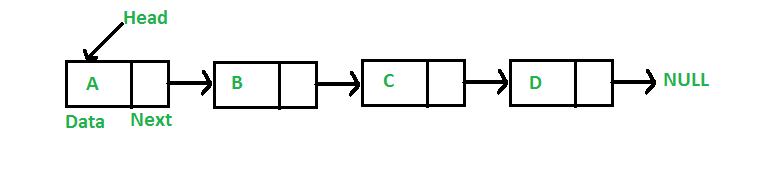
\includegraphics[width=10cm]{Linkedlist.png}
                \caption{Modelo de las listas enlazadas.}
                \label{fig:linked}
            \end{figure}
            \section{Métodos usados}
            Como cualquier clase, estos contienen distintos métodos, propiedades y constructores, de los cuales los mas relevantes son los siguientes:
            \subsection{Constructores}
            \begin{itemize}
                \item \emph{List\(<\!T\!>\)(): }Inicializa una nueva instancia de la clase que está vacia y tiene la capacidad inicial por defecto.
                \item \emph{List\(<\!T\!>\)(IEnumerable\(<\!T\!>\)): }Inicializa una nueva instancia de la clase que contiene elementos copiados de una colección especificada\\
                y ue tiene la capacidad suficiente para acomodar el número de elementos copiados.
                \item \emph{List\(<\!T\!>\)(Int32): }Inicializa una nueva instancia de la clase la cual está vacia y tiene la capacidad inicial especificada.
            \end{itemize}
            \subsection{Propiedades}
            \begin{itemize}
                \item \emph{Capacity: }obtiene o establece el numero total de elementos que la estructura interna puede mantener sin un cambio de tamaño.
                \item \emph{Count: }obtiene el numero de elementos contenidos en \emph{List\(<\!T\!>\).}
                \item \emph{Item[Int32]: }obtiene o establece el elemento del índice especificado.
            \end{itemize}
            \subsection{Métodos}
            \begin{itemize}
                \item \emph{Add(T): }añade un objeto al final de la lista.
                \item \emph{Clear(): }remueve todos los elementos de la lista.
                \item \emph{Contains(T): }determina si un elemento dado está dentro de la lista.
                \item \emph{IndexOf(T, Int32): }busca el índice de la primer ocurrencia entre el rango de elementos desde dicho indice hasta el final de la lista.
                \item \emph{Remove(T): }remueve la primer ocurrencia del objeto especificado en la lista. 
            \end{itemize}
            \section{Conclusión}
            El uso de esta clase permite el desarrollo de programas más sencillos de desarrollar y por ende mas sencillos de comprender para el aprendizaje de los mismos.
        \end{justify}

    %bibliografía
    \newpage
    \lhead{}
    \addcontentsline{toc}{section}{Referencias}
    \printbibliography
\end{document}